\documentclass[12pt]{article}

\usepackage{sbc-template}
\usepackage{graphicx,url}
\usepackage[hidelinks]{hyperref}
\usepackage[brazil]{babel}
\usepackage[utf8]{inputenc}
\usepackage{booktabs}
\usepackage{longtable}
\usepackage{array}
\usepackage{ragged2e}
\usepackage{float}
\setlength{\textfloatsep}{8pt}
\setlength{\intextsep}{8pt}
\setlength{\abovecaptionskip}{4pt}

\sloppy

\title{Mineração de métricas DORA em repositórios open-source populares:\\
o que acontece quando os proxies são validados}

\author{Guilherme Costa\inst{1}, Henrique Jardim Melo\inst{1}, Gabriel Afonso\inst{1}}

\address{Engenharia de Software -- Pontifícia Universidade Católica de Minas Gerais
  (PUC Minas)\\
  Belo Horizonte -- MG -- Brasil
  \email{\{guilherme,henrique,gabriel\}@sga.pucminas.br}
}

\begin{document}

\maketitle

\begin{abstract}
We mine the four DORA metrics from 900 popular open-source repositories that use
GitHub Actions, and then test whether the proxies required to do so are valid
measures. Three raters independently labelled 300 releases: no version of the
corrective-release heuristic reaches the required F1 of 0.70, and the one behind
the dataset has 36.5\% precision. Conditioning on observation opportunity, the
correlation between deployment frequency and change failure rate collapses from
0.604 to $-0.039$, showing that this proxy largely measures publication cadence
rather than failure. The DORA bands show no discriminant power against repository
attributes. Estimates reproduce across three independent samples.
\end{abstract}

\begin{resumo}
Minera-se as quatro métricas DORA de 900 repositórios open-source populares que
usam GitHub Actions e, em seguida, testa-se se os proxies necessários para isso
são medidas válidas. Três avaliadores rotularam 300 releases de forma
independente: nenhuma versão da heurística de release corretiva alcança o F1
mínimo de 0,70, e a que gerou o dataset tem precisão de 36,5\%. Ao condicionar
pela oportunidade de observação, a correlação entre frequência de deploy e taxa
de falha cai de 0,604 para $-0,039$, mostrando que esse proxy mede, em boa parte,
cadência de publicação e não falha. As faixas DORA não apresentam poder
discriminante. As estimativas se reproduzem em três amostras independentes.
\end{resumo}

\section{Introdução}

\subsection{Contexto e problema}

As quatro métricas DORA — frequência de deploy, lead time for changes, change failure rate e tempo de recuperação — viraram o vocabulário padrão para falar de desempenho de entrega de software, e sua tese central é que velocidade e estabilidade não são um trade-off. Elas foram definidas, porém, para equipes que controlam o próprio pipeline de produção e sabem, por definição operacional interna, o que conta como ``deploy'' e o que conta como ``falha em produção''.

Repositórios open-source no GitHub não oferecem nenhuma das duas coisas. Não há registro de implantação, não há registro de incidente e não há a quem perguntar. O que existe são rastros: releases publicadas, execuções de workflow, commits e tags. Medir DORA aqui, portanto, não é aplicar uma definição — é \textbf{escolher proxies} e herdar o erro de cada escolha. Uma release é um deploy? Uma execução de CI que falha é uma falha em produção? Uma release de \emph{patch} publicada três dias depois da anterior corrige um defeito, ou é rotina?

Cada resposta é uma hipótese não verificada ligando um atributo interno, que se consegue contar, a um atributo externo, que é o que interessa. Calcular as quatro métricas numa amostra grande é a parte mecânica; a parte que decide se os números significam alguma coisa é perguntar \textbf{o quanto os proxies são medidas válidas} — se concordam com julgamento humano, se sobrevivem à troca da definição, se se reproduzem em amostras independentes e se as faixas separam grupos distintos.

\subsection{Objetivo e questões de pesquisa}

O objetivo é minerar as métricas DORA de repositórios populares que usam GitHub Actions e, em paralelo, avaliar a validade das medidas. O escopo do enunciado é de 300 repositórios; este trabalho o estende para \textbf{900}, em três amostras independentes, para poder testar reprodutibilidade.

\begin{table}[!htbp]
\centering
\scriptsize
\begin{tabular}{p{0.087\columnwidth}p{0.773\columnwidth}}
\toprule
\textbf{RQ} & \textbf{Pergunta} \\
\midrule
\textbf{RQ01} & Qual a frequência de deploys dos repositórios populares que usam CI/CD? \\
\textbf{RQ02} & Qual o tempo entre um commit e seu respectivo deploy? \\
\textbf{RQ03} & Qual a taxa de falha das mudanças entregues? \\
\textbf{RQ04} & Qual o tempo de recuperação após uma execução de CI/CD com falha? \\
\textbf{RQ05} & Maior frequência de deploy se associa a maior ou menor taxa de falha? \\
\textbf{RQ06} & Quais características dos repositórios se associam a melhor desempenho? \\
\textbf{RQ07} & O quanto a classificação DORA depende da definição operacional? \\
\bottomrule
\end{tabular}
\end{table}

A RQ08 (bônus) trata da evolução temporal das métricas dentro da janela.

\subsection{Hipóteses informais}

Uma hipótese por RQ, com a origem de cada uma declarada. ``Origem'' diz de onde veio a expectativa — não dos dados deste trabalho (ver a nota de registro em 1.5).

\begin{table}[!htbp]
\centering
\scriptsize
\begin{tabular}{p{0.066\columnwidth}p{0.292\columnwidth}p{0.502\columnwidth}}
\toprule
\textbf{\#} & \textbf{Hipótese} & \textbf{Origem da expectativa} \\
\midrule
\textbf{H01} & Os repositórios entregam com alta frequência: mediana de \textbf{pelo menos uma release por semana}. & O programa DORA trata entrega frequente como marca de maturidade, e o critério de inclusão ($\geq$ 5 releases e $\geq$ 50 workflow runs na janela) já seleciona projetos ativos. \\
\textbf{H02} & O lead time mediano fica \textbf{na casa dos dias, não das horas}, e a variante (a), por release, é \textbf{sistematicamente maior} que a (b), por commit. & A primeira parte vem do contraste entre o padrão Elite do DORA (< 1 dia) e o ritmo assíncrono e voluntário do open source. A segunda vem da própria dica do enunciado na RQ02: um commit antigo ``esquecido'' numa release faz a (a) explodir e pouco afeta a (b). \\
\textbf{H03} & A taxa de falha fica \textbf{abaixo de 15\%} nas duas variantes, e as duas chegam a \textbf{valores próximos}. & 15\% é o limiar DORA que separa Elite/High do resto. A expectativa de convergência vem de supor que as duas variantes medem o mesmo construto por caminhos diferentes — que é exatamente a suposição que o trabalho precisa testar. \\
\textbf{H04} & O tempo mediano de recuperação fica \textbf{abaixo de 24 horas}. & Um pipeline de CI quebrado bloqueia todo mundo que depende dele; a expectativa é que consertá-lo seja prioridade imediata. O padrão Elite do DORA é menos de uma hora. \\
\textbf{H05} & A correlação entre frequência de deploy e CFR é \textbf{nula ou negativa}. & É a tese central do DORA, citada no próprio enunciado da RQ05: velocidade e estabilidade não são um trade-off, e quem entrega mais não falha mais. \\
\textbf{H06} & Repositórios mais populares, com mais contribuidores e mais antigos têm \textbf{desempenho DORA melhor}, com efeito ao menos pequeno ($\varepsilon$$^2$ $\geq$ 0,01). & Mais gente e mais maturidade deveriam significar mais automação, mais processo e mais disciplina de release. \\
\textbf{H07} & A classificação DORA é \textbf{majoritariamente estável} à definição operacional: \textbf{menos de 20\%} dos repositórios mudam de faixa entre duas combinações. & Se as faixas medem um atributo real do repositório, e não um artefato do proxy, trocar a definição não deveria reclassificar a maioria. \\
\bottomrule
\end{tabular}
\end{table}

\subsection{Nota sobre o registro das hipóteses}

O protocolo correto registra as hipóteses \textbf{antes} da coleta, e aqui isso não aconteceu: o Lab03 começou em 08/10/2026, o primeiro dataset entrou em 13/10/2026 e as hipóteses acima foram escritas em \textbf{20/10/2026}, com os resultados já disponíveis. Elas são \textbf{reconstruídas}, não pré-registradas.

Para que a reconstrução não seja racionalização do que foi encontrado, cada hipótese declara a origem da expectativa, e nenhuma foi derivada dos resultados. O leitor audita isso pelo saldo: \textbf{cinco das sete foram refutadas} (seção 4). Hipóteses escritas depois do resultado tendem a acertar; estas, na maioria, erram. A seção 5.4 trata disso como ameaça aberta.

\subsection{Contribuições}

Um \textbf{dataset público de 900 repositórios} com as quatro métricas e os eventos brutos; uma \textbf{avaliação de validade} segundo os seis critérios da IEEE 1061, e não apenas o cálculo das métricas; a demonstração, por duas vias independentes, de que \textbf{o CFR na variante (b) não mede falha} (seções 2.7 e 3.7); a evidência de que as \textbf{faixas DORA não têm poder discriminante} nesta população, com um índice contínuo como alternativa; e um \textbf{ajuste de distribuições} que mostra por que média e desvio-padrão não se aplicam aqui.

As seções seguintes tratam de metodologia e validação manual (2), resultados das RQs e análises de validade (3), hipóteses contra resultados (4), ameaças à validade (5) e pacote de replicação (6).


\section{Metodologia}

\subsection{Fonte de dados}

Os dados vêm da API pública do GitHub e foram coletados por um script próprio do grupo, sem bibliotecas prontas de acesso à API. O script usa a API REST para busca, releases, comparações entre releases e workflow runs, e a GraphQL para as tags com data. O pipeline inteiro roda com um único comando (\texttt{python -m pipeline --config config.yaml}). Cada resposta da API fica em cache local, então interromper a coleta e rodá-la de novo continua de onde parou e reproduz o mesmo dataset sem novas chamadas. O cliente HTTP respeita os cabeçalhos de rate limit e repete com \emph{backoff} exponencial as respostas 5xx e as falhas de rede.

\subsection{Janela de observação}

A janela tem 12 meses, de \textbf{1º de outubro de 2025 a 30 de setembro de 2026} \textbf{[PENDENTE: confirmar com as datas fixadas pelo professor]}. Isso dá aproximadamente 52,1 semanas. Só entram nas métricas as releases publicadas e os workflow runs criados dentro dela. A exceção é a release imediatamente anterior a uma release da janela, que é usada como base para obter os commits incluídos, mesmo estando fora.

\subsection{Seleção dos repositórios e funil}

A busca cobriu repositórios com mais de 1.000 estrelas, não arquivados e com \emph{push} depois do início da janela. Como cada consulta devolve no máximo 1.000 resultados, ela foi fatiada em nove faixas de estrelas. Os candidatos foram embaralhados com semente fixa e avaliados nessa ordem até a amostra chegar a 300, de modo que ela não se concentre nos mais estrelados de cada faixa. Os filtros, aplicados do mais barato ao mais caro, são: (i) usa GitHub Actions; (ii) tem ao menos 5 releases publicadas, sem pré-release, na janela; (iii) tem ao menos 50 workflow runs válidos disparados por \emph{push} no \emph{default branch}.

\textbf{Tabela 1 — Funil de seleção} (\texttt{data/funil.csv}).

\begin{table}[!htbp]
\centering
\scriptsize
\begin{tabular}{lrrl}
\toprule
\textbf{Etapa} & \textbf{Restantes} & \textbf{Descartados} & \textbf{Motivo} \\
\midrule
Candidatos da busca & 8.457 & — & — \\
Avaliados (ordem aleatória) & 1.108 & 7.349 & alvo de 300 já atingido \\
Usam GitHub Actions & 937 & 171 & nenhum workflow cadastrado \\
$\geq$ 5 releases na janela & 399 & 538 & menos de 5 releases \\
$\geq$ 50 runs válidos & 300 & 99 & menos de 50 runs em \texttt{push} \\
\bottomrule
\end{tabular}
\end{table}

O filtro mais restritivo é o de releases: \textbf{57\% dos repositórios que usam Actions publicaram menos de 5 releases em 12 meses}, o que indica que muitos projetos populares entregam por \emph{rolling release}, publicação direta em registros de pacotes ou sem versionamento formal. Como cada faixa contribui no máximo com seus 1.000 mais estrelados, a amostra fica deslocada para repositórios populares: mediana de 9.485 estrelas (IQR 2.844–28.694).

\subsection{Definições operacionais}

Seguem a seção 3 do enunciado, comum à turma. \textbf{Deploy} é release publicada (\texttt{draft = false}), sem pré-release, datada por \texttt{published\_at}. \textbf{Execuções de CI} são workflow runs do \emph{default branch} com \texttt{event = push}; \texttt{success} conta como sucesso, \texttt{failure}, \texttt{timed\_out} e \texttt{startup\_failure} como falha, e os demais valores são ignorados.

\begin{itemize}
  \item \textbf{Frequência (RQ01):} deploys na janela ÷ semanas da janela.
  \item \textbf{Lead time (RQ02):} os commits de cada deploy D vêm de \texttt{compare/\{anterior\}...\{D\}}. Variante \textbf{(a)}, por release: \texttt{data(D) -- commit mais antigo de D}, com mediana entre deploys. Variante \textbf{(b)}, por commit: \texttt{data(D) -- data de cada commit}, com mediana de todos. Ficam fora o primeiro deploy da história, os \emph{compare} 404 e os com mais de 1.000 commits ou recusados pela API — quase sempre comparações entre linhas de versão distintas, que não representam o que entrou no deploy.
  \item \textbf{CFR (RQ03):} variante \textbf{(a)}, falhas ÷ (falhas + sucessos) de CI; variante \textbf{(b)}, o deploy falhou se um deploy corretivo saiu em até 7 dias, com os últimos 7 dias da janela fora do denominador (censura). O dataset usa a heurística \textbf{v0} (SemVer: sobe só o \emph{patch}). Outras três foram implementadas e comparadas: \textbf{v1} (metade dos commits é \texttt{fix}/\texttt{revert}), \textbf{v2} (v0 e no máximo 3 commits) e \textbf{v3} (v0, v1 ou tag com \texttt{hotfix}/\texttt{patch}). As quatro divergem muito entre si — a v0 marca 8.186 releases como corretivas, a v1 apenas 1.479 — o que já indicava a necessidade de validação humana. A escolha final está na seção 2.7: \textbf{nenhuma atinge o F1 mínimo}, e a v0 foi mantida como referência.
  \item \textbf{Recuperação (RQ04):} runs agrupados por workflow e ordenados por \texttt{run\_started\_at}. Um episódio começa na primeira falha após um sucesso e termina no sucesso seguinte, com duração \texttt{updated\_at(sucesso) -- run\_started\_at(1ª falha)}; o valor do repositório é a mediana dos episódios fechados. Episódios sem sucesso até o fim da janela são \textbf{censurados} e contados à parte. Falhas anteriores ao primeiro sucesso não abrem episódio.
\end{itemize}

\subsection{Variantes para a análise de sensibilidade (RQ 07)}

As métricas de velocidade e o CFR (b) são calculados para três unidades de deploy:

\begin{table}[!htbp]
\centering
\scriptsize
\begin{tabular}{p{0.195\columnwidth}p{0.364\columnwidth}p{0.301\columnwidth}}
\toprule
\textbf{Unidade} & \textbf{Definição} & \textbf{Data} \\
\midrule
\texttt{release} (referência) & Release publicada sem pré-release & \texttt{published\_at} \\
\texttt{release\_pre} & Release publicada, incluindo pré-releases & \texttt{published\_at} \\
\texttt{tag} & Tag do repositório & Data de autoria do commit apontado \\
\bottomrule
\end{tabular}
\end{table}

Para não esgotar a cota, o lead time de uma unidade não é calculado quando ela tem mais de 300 deploys na janela. Isso acontece sobretudo com tags em monorepos. Esses casos ficam marcados na coluna \texttt{lt\_<unidade>\_omitido}. As combinações C1–C3 da RQ 07 são montadas a partir dessas colunas na S03 (\#142).

\subsection{Dataset e viés de seleção}

O dataset final (\texttt{data/dataset\_dora.csv}) tem uma linha por repositório, com os metadados da RQ06, as métricas em todas as variantes e as contagens de qualidade da coleta. Cada coluna está descrita em \texttt{data/DICIONARIO.md}.

A amostra 1 tem 300 repositórios em 27 linguagens, idade mediana de 5,8 anos (IQR 2,0–10,9) e 142 contribuidores medianos (IQR 50–335); a coleta somou 17.217 releases e 833.582 workflow runs válidos. Perdas conhecidas: 244 releases ficaram fora do lead time por \emph{compare} acima de 1.000 commits ou recusado pela API, 8 por \emph{compare} 404, 7 repositórios tiveram o lead time omitido por excederem 300 releases na janela, e 139 de 20.077 episódios de falha ficaram censurados.

O viés de seleção foi medido comparando os aceitos com cada etapa de descarte (Mann-Whitney e delta de Cliff para estrelas e idade, qui-quadrado para linguagem, com Holm). \textbf{Os aceitos têm mais estrelas que os descartados} (9.484,5 contra 2.969,5; $\delta$ = 0,292, efeito pequeno; p < 0,001) e são ligeiramente mais jovens ($\delta$ = --0,116, desprezível; p = 0,016), e a distribuição de linguagens difere (p < 0,001). O filtro de Actions é o mais seletivo ($\delta$ de estrelas = 0,357). A amostra caracteriza, portanto, \textbf{projetos populares, ativos e que publicam releases com frequência} — não o ecossistema open-source em geral.

Dois testes de sanidade não encontraram diferença: os 1.108 candidatos avaliados contra os 7.349 não avaliados ($\delta$ $\leq$ 0,017; p = 1) e a A1 contra a A2 ($\delta$ $\leq$ 0,019; p = 1). A ordem de avaliação e a composição das amostras não introduzem viés adicional, o que não remove o viés dos critérios de inclusão (seção 5.3). Tudo se regenera com \texttt{python -m analise.caracterizacao}.

\subsection{Validação manual (amostra-ouro)}

\textbf{Sorteio.} Foram sorteados 60 repositórios da amostra 1 com semente fixa (\texttt{sample(n=60, random\_state=42)}) e, para cada um, até 5 releases da janela com um \texttt{random.Random(42)} novo por repositório, num total de 300 releases. O sorteio é reprodutível por \texttt{python -m analise.amostra\_ouro} e a lista está em \texttt{validacao/amostra\_ouro\_repos.csv} e \texttt{validacao/amostra\_ouro\_releases.csv}.

\textbf{Rotulagem independente.} Os três integrantes rotularam sozinhos, sem consultar os demais nem ver a saída da heurística, três dimensões: (i) tipo do projeto; (ii) se as releases representam entregas reais ao usuário; (iii) se cada release sorteada é corretiva. São 360 julgamentos por pessoa, 1.080 no total, em \texttt{validacao/rotulos\_<nome>\_*.csv}.

\textbf{Concordância.} Medida pelo kappa de Fleiss por dimensão (Tabela 4), interpretada segundo Landis e Koch (1977). A concordância bruta é reportada junto porque o kappa desconta a concordância esperada por acaso e, quando uma categoria domina, pode colapsar mesmo com acordo alto — é o que ocorre em \texttt{releases\_reais}.

\textbf{Tabela 4 — Concordância entre os três avaliadores.}

\begin{table}[!htbp]
\centering
\scriptsize
\begin{tabular}{lrrlrrl}
\toprule
\textbf{Dimensão} & \textbf{n} & \textbf{$\kappa$ de Fleiss} & \textbf{Interpretação} & \textbf{Os 3 iguais} & \textbf{Maioria 2/3} & \textbf{Categoria dominante} \\
\midrule
Tipo do projeto & 60 & 0,872 & quase perfeita & 86,7\% & 100\% & aplicação/serviço (41,7\%) \\
Releases são entrega real & 60 & 0,157 & leve & 90,0\% & 98,3\% & sim (95,6\%) \\
Release é corretiva & 300 & 0,504 & moderada & 71,0\% & 100\% & não (73,4\%) \\
\bottomrule
\end{tabular}
\end{table}

O $\kappa$ de 0,157 em \texttt{releases\_reais} \textbf{não} significa desacordo: os três concordaram em 90\% dos repositórios. Significa que quase todos os repositórios receberam o mesmo rótulo (\texttt{sim} em 95,6\% dos julgamentos), de modo que o acaso já explicaria quase toda a concordância observada. A medida é pouco informativa nessa dimensão, e a leitura correta é a concordância bruta.

O $\kappa$ de 0,504 em \texttt{corretiva} é o número que importa, e é apenas moderado. Três pessoas lendo as mesmas notas de release e a mesma lista de commits divergiram em 29\% dos casos. A prevalência de ``sim'' variou de 16,7\% a 37,3\% entre avaliadores. Isso é evidência direta de que \textbf{o próprio conceito de ``release corretiva'' é ambíguo}, e não apenas difícil de automatizar.

\textbf{Consenso.} Resolvido por maioria de 2 em 3, com o protocolo em \texttt{validacao/PROTOCOLO.md}. Houve maioria em 100\% das releases e dos tipos de projeto; apenas 1 repositório ficou sem maioria em \texttt{releases\_reais} e segue marcado para decisão em reunião. O gabarito final tem 78 releases corretivas e 222 não corretivas (26,0\% de prevalência), em \texttt{validacao/consenso\_releases.csv}.

\textbf{Avaliação da heurística.} Quatro versões foram testadas contra o consenso (Tabela 5). \textbf{Nenhuma atinge o F1 mínimo de 0,70 exigido pelo enunciado.}

\textbf{Tabela 5 — Heurística de release corretiva contra o gabarito humano (n = 300).}

\begin{table}[!htbp]
\centering
\scriptsize
\begin{tabular}{p{0.232\columnwidth}p{0.408\columnwidth}p{0.068\columnwidth}p{0.068\columnwidth}p{0.084\columnwidth}}
\toprule
\textbf{Versão} & \textbf{Regra} & \textbf{Precisão} & \textbf{Recall} & \textbf{F1} \\
\midrule
v0 \texttt{semver\_patch} & sobe só o \emph{patch} da versão & 36,5\% & 69,2\% & 0,478 \\
v1 \texttt{mensagens} & $\geq$ metade dos commits é \texttt{fix:}/revert & 94,4\% & 21,8\% & 0,354 \\
v2 \texttt{patch\_poucos\_commits} & v0 \textbf{e} $\leq$ 3 commits & 59,5\% & 28,2\% & 0,383 \\
\textbf{v3 \texttt{combinada}} & v0 \textbf{ou} v1 \textbf{ou} tag com \texttt{hotfix}/\texttt{patch} & 37,7\% & 73,1\% & \textbf{0,498} \\
\bottomrule
\end{tabular}
\end{table}

A v0, que gerou o \texttt{cfr\_b\_release} de todo o dataset, tem \textbf{precisão de 36,5\%}: de cada três releases que ela marca como corretivas, duas não são, segundo o consenso humano. A v1 inverte o erro — precisão de 94,4\% com recall de 21,8\%, ou seja, quando acusa quase sempre acerta, mas deixa passar quatro de cada cinco correções reais. A v3, melhor por F1, supera a v0 por apenas 0,020, e as duas produzem medianas de CFR (b) praticamente iguais (25,0\% em ambas).

Por isso \textbf{a v0 foi mantida como definição de referência}: trocá-la pela v3 exigiria recalcular as três amostras sem ganho de validade mensurável. A decisão e seu custo estão registrados aqui e discutidos na seção 5.1, onde a validade de construto do CFR (b) deixa de ser uma suspeita e passa a ser um resultado medido. As quatro versões e o detalhamento estão em \texttt{validacao/heuristica\_versoes.md} e \texttt{validacao/avaliacao\_heuristica.csv}.


\section{Resultados}

Todas as métricas são resumidas por \textbf{mediana e IQR} (1º–3º quartil), como pede o enunciado e como a seção 3.7.5 demonstra ser necessário. Os resultados aparecem no escopo pedido (300 repositórios da amostra 1) e na amostra estendida, para mostrar que não dependem do sorteio.

O CFR (b) usa a heurística v0 de release corretiva, \textbf{reprovada na validação contra o gabarito humano} (F1 = 0,478, precisão 36,5\%; seção 2.7). Foi mantida por ser a melhor disponível sem recoletar, e todo resultado marcado \textbf{[NÃO VALIDADO]} deve ser lido com essa ressalva.

\textbf{Tabela 3 — Resumo das métricas.} Mediana [IQR].

\begin{table}[!htbp]
\centering
\scriptsize
\begin{tabular}{p{0.387\columnwidth}p{0.087\columnwidth}p{0.193\columnwidth}p{0.193\columnwidth}}
\toprule
\textbf{Métrica} & \textbf{n (300 / 900)} & \textbf{300} & \textbf{900} \\
\midrule
Frequência de deploy (releases/semana) & 300 / 900 & 0,35 [0,19 – 0,81] & 0,35 [0,19 – 0,84] \\
Lead time (a), por release (dias) & 293 / 873 & 13,2 [3,1 – 37,3] & 12,0 [3,0 – 37,4] \\
Lead time (b), por commit (dias) & 293 / 873 & 8,8 [2,8 – 29,4] & 9,0 [2,5 – 28,1] \\
CFR (a), proxy de CI & 300 / 900 & 5,6\% [2,2\% – 11,2\%] & 5,3\% [2,2\% – 11,2\%] \\
CFR (b), proxy de entrega [NÃO VALIDADO] & 300 / 900 & 25,0\% [5,2\% – 56,5\%] & 25,0\% [6,2\% – 50,3\%] \\
Tempo de recuperação (horas) & 278 / 834 & 2,8 [0,9 – 11,9] & 3,1 [0,9 – 17,3] \\
\bottomrule
\end{tabular}
\end{table}

Ficam sem lead time os repositórios com mais de 300 releases na janela, cujo cálculo foi omitido para preservar a cota da API (7 na A1, 27 no total). Ficam sem tempo de recuperação os que não tiveram nenhum episódio de falha fechado (22 na A1, 66 no total).

\textbf{Leitura geral:} ao triplicar a amostra, \textbf{todas as medianas ficam praticamente no mesmo lugar}, dentro do intervalo de confiança do escopo de 300. O detalhe está na seção 3.7.1. As figuras se regeneram com \texttt{python -m analise}.

\subsection{RQ 01 a RQ 04 — as quatro métricas}

Os valores centrais estão na Tabela 3. Em síntese:

\textbf{Frequência (RQ01).} Mediana de 0,35 release por semana, cerca de uma a cada 20 dias. Quase metade dos repositórios é \textbf{Medium} (entre uma por mês e uma por semana) e um terço é \textbf{Low}. Só 2\% alcançam Elite. Projetos que entregam continuamente sem publicar releases ficam subestimados por construção, e os que não chegam a 5 releases já caíram no funil.

\textbf{Lead time (RQ02).} Medianas de 13,2 dias pela variante (a) e 8,8 pela (b). Em \textbf{65\% dos repositórios a (b) é menor}. A razão é estrutural: a (a) mede desde o commit \emph{mais antigo} de cada release, e um único commit esquecido puxa a release inteira para cima; a (b) usa a mediana de todos os commits, e a maioria entra perto da publicação. Quando cada release tem poucos commits, as duas convergem.

\textbf{Change failure rate (RQ03).} Os dois proxies contam histórias opostas. Pela falha de CI, \textbf{84\% dos repositórios são Elite} (mediana 5,6\%). Pela release corretiva em até 7 dias, só \textbf{37\%} (mediana 25,0\%), e 23\% têm CFR (b) igual a zero. O CFR (a) mede falha de \emph{pipeline} — teste instável entra como falha; o CFR (b) depende da heurística corretiva, reprovada na seção 2.7.

\textbf{Recuperação (RQ04).} Mediana de 2,8 horas. Recuperam-se em menos de 1 hora 27\% dos repositórios, em menos de 1 dia 83\%, em menos de 1 semana 97\%. Os episódios censurados são 0,7\% de 20.077.

\begin{figure}[!htbp]
\centering
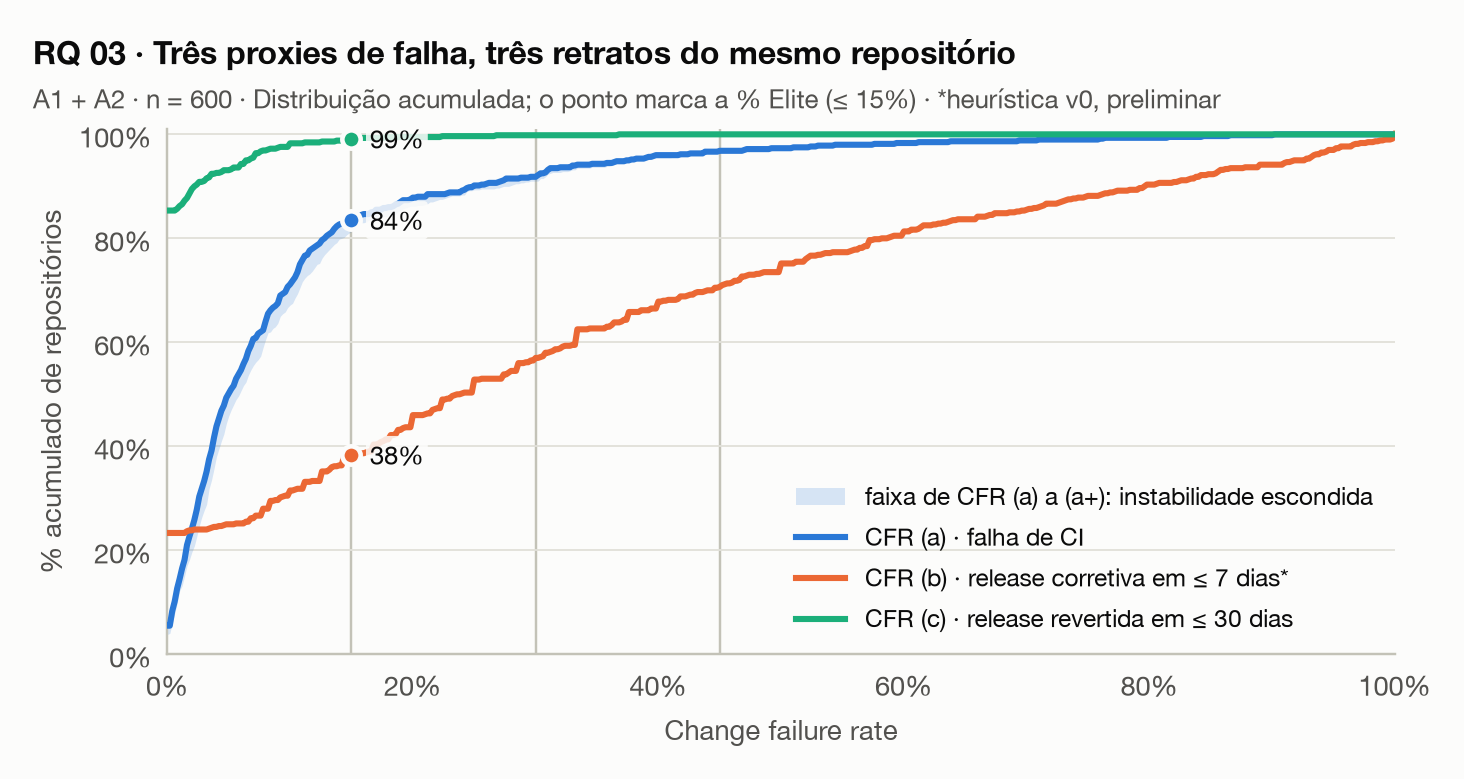
\includegraphics[width=0.55\columnwidth]{figuras/a600_fig04_rq03_cfr.png}
\caption{Change failure rate pelos dois proxies}
\end{figure}

\textbf{Como ler.} Curva acumulada: para cada valor de CFR no eixo horizontal, a altura é a proporção de repositórios com CFR até ali. Quanto mais cedo a curva sobe, menor a taxa de falha. As verticais são as fronteiras DORA (15\%, 30\%, 45\%). As duas curvas separadas são o resultado: o proxy escolhido domina a resposta da RQ03.

\subsection{Classificação DORA (combinação de referência)}

\begin{figure}[!htbp]
\centering
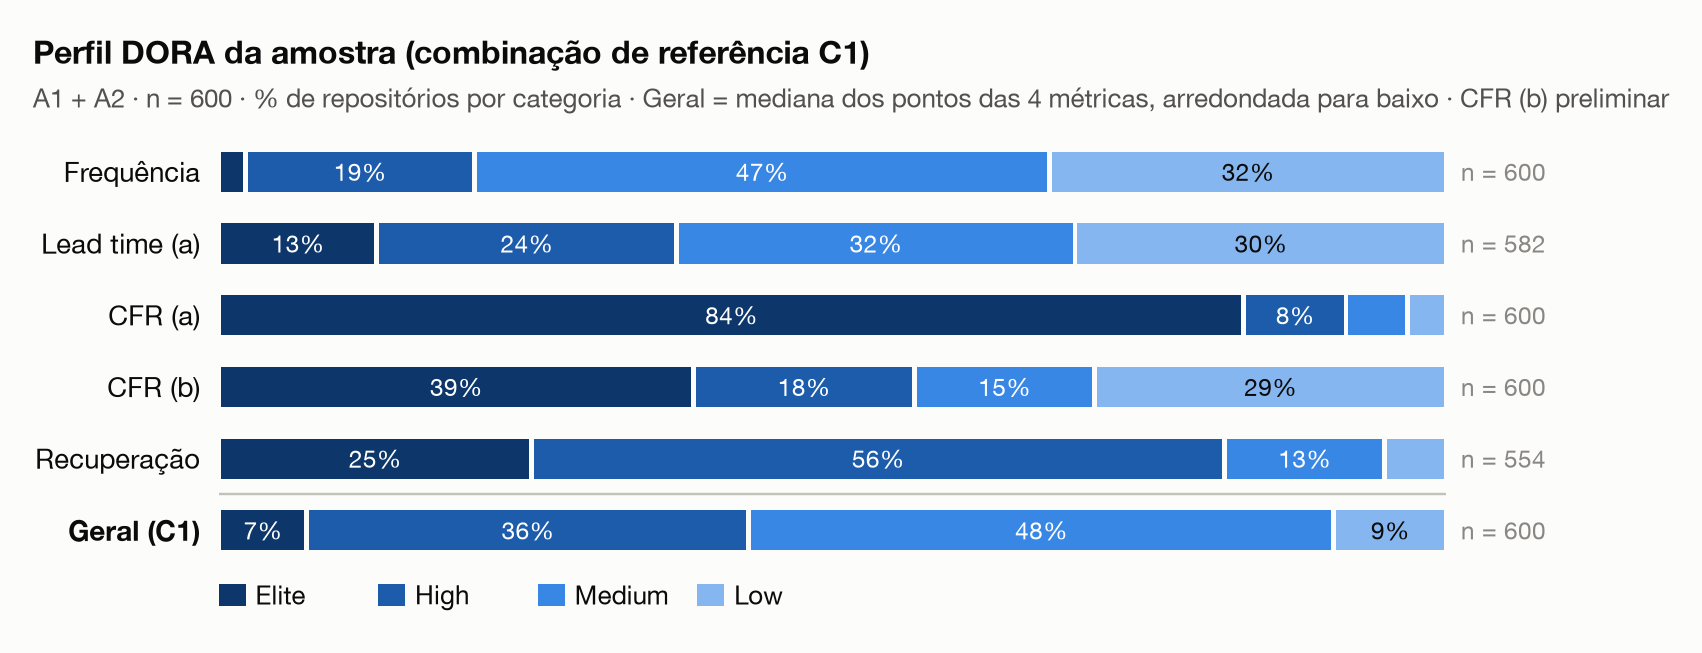
\includegraphics[width=0.55\columnwidth]{figuras/a600_fig06_perfil_dora.png}
\caption{Perfil DORA por métrica}
\end{figure}

\textbf{Como ler.} Cada barra soma 100\% dos repositórios, divididos pela categoria DORA daquela métrica; o tom mais escuro é Elite. ``Geral'' é a classificação final do enunciado: mediana dos pontos das quatro métricas, arredondada para baixo.

\begin{table}[!htbp]
\centering
\scriptsize
\begin{tabular}{lrrrr}
\toprule
\textbf{Classificação geral} & \textbf{Elite} & \textbf{High} & \textbf{Medium} & \textbf{Low} \\
\midrule
300 repositórios & 8\% & 35\% & 50\% & 7\% \\
600 repositórios & 7\% & 36\% & 48\% & 9\% \\
\bottomrule
\end{tabular}
\end{table}

Metade é Medium e um terço é High. Cada métrica puxa para um lado: o CFR (a), quase todo em Elite, puxa para cima; a frequência, com \textasciitilde{}80\% entre Medium e Low, puxa para baixo; o lead time se espalha pelas quatro.

\subsection{RQ 05 — Velocidade $\times$ estabilidade}

\begin{figure}[!htbp]
\centering
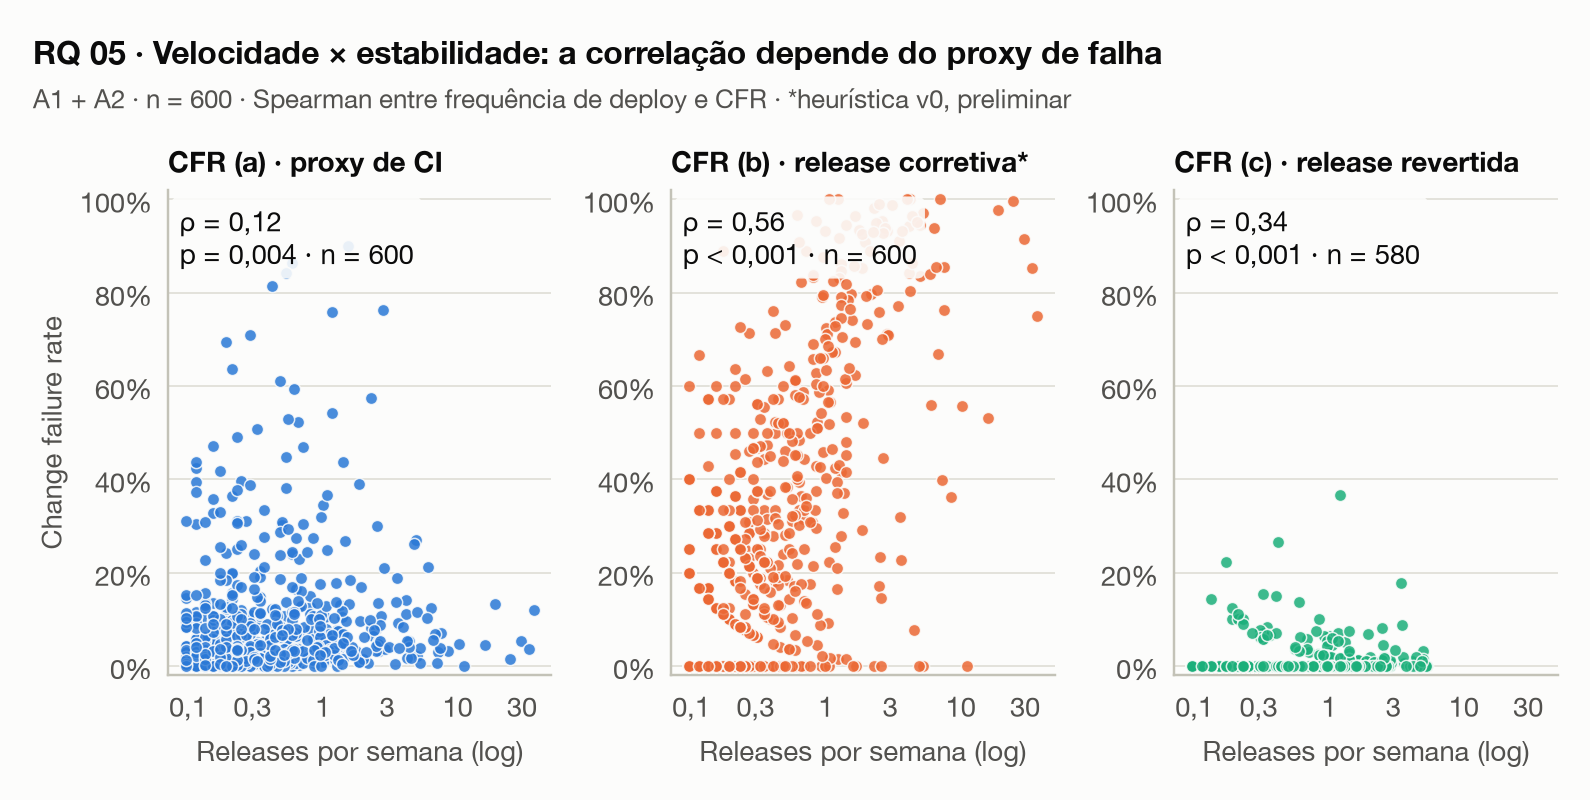
\includegraphics[width=0.55\columnwidth]{figuras/a600_fig07_rq05_velocidade_estabilidade.png}
\caption{Frequência de deploy contra taxa de falha}
\end{figure}

\textbf{Como ler.} Cada ponto é um repositório: frequência de deploy no eixo horizontal (escala log), CFR no vertical. O $\rho$ de Spearman vai de --1 a 1; perto de zero indica ausência de relação monotônica.

\begin{table}[!htbp]
\centering
\scriptsize
\begin{tabular}{p{0.430\columnwidth}p{0.215\columnwidth}p{0.215\columnwidth}}
\toprule
\textbf{Correlação com a frequência} & \textbf{300} & \textbf{600} \\
\midrule
CFR (a), proxy de CI & $\rho$ = 0,18 (p = 0,002) & $\rho$ = 0,12 (p = 0,004) \\
CFR (b), proxy de entrega [NÃO VALIDADO] & $\rho$ = 0,60 (p < 0,001) & $\rho$ = 0,56 (p < 0,001) \\
\bottomrule
\end{tabular}
\end{table}

Pelo CI a correlação é significativa mas \textbf{fraca}, e diminui com a amostra maior: publicar mais não se associa a quebrar mais o pipeline, o que é coerente com a tese do DORA. Pela entrega é \textbf{forte} — mas a seção 3.7 mostra que isso é artefato da definição, não achado. Em nenhum dos casos correlação implica causalidade.

\subsection{RQ 06 — Características associadas ao desempenho}

\begin{figure}[!htbp]
\centering
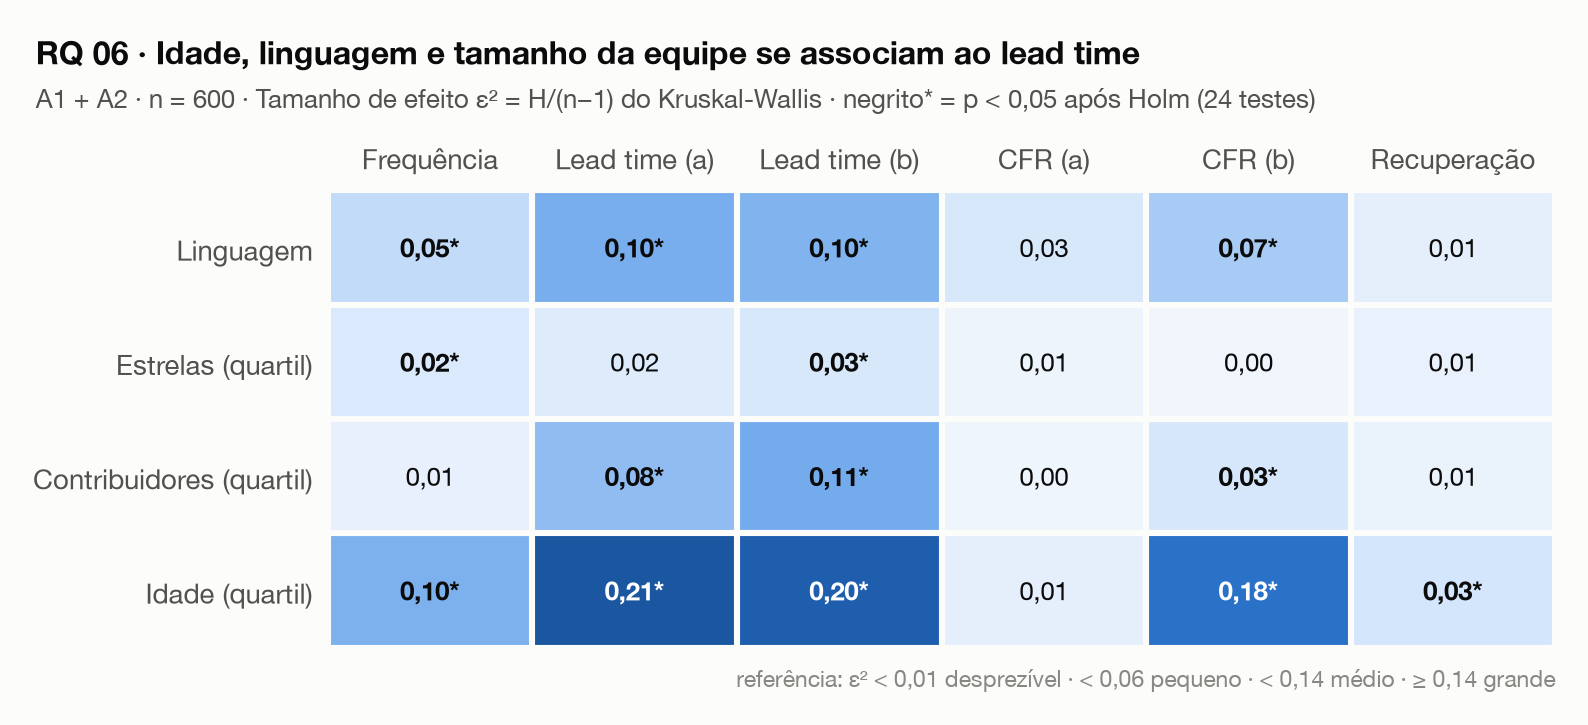
\includegraphics[width=0.55\columnwidth]{figuras/a600_fig08_rq06_fatores.png}
\caption{Tamanho de efeito por fator e métrica}
\end{figure}

\textbf{Como ler.} Cada célula cruza uma característica do repositório com uma métrica. O valor é o tamanho de efeito $\varepsilon$$^2$ = H/(n--1) do Kruskal-Wallis: quanto da variação da métrica aquela característica explica (< 0,01 desprezível, < 0,06 pequeno, < 0,14 médio, $\geq$ 0,14 grande). Em negrito, os que sobrevivem à correção de Holm sobre os 24 testes.

\textbf{A idade é o fator de maior efeito} ($\varepsilon$$^2$ = 0,21–0,25 no lead time, efeito grande): repositórios de até 2 anos têm lead time mediano de 2,0 dias contra 28,5 nos mais antigos, e publicam quase três vezes mais (0,67 contra 0,23 release/semana). Equipes maiores têm lead time maior ($\varepsilon$$^2$ 0,08–0,14). O \textbf{CFR (a) não se associa a nenhum fator}.

\textbf{A linguagem só fica significativa com 600 repositórios} — com 300 não sobrevivia a Holm. Lead time mediano: TypeScript 7,1 dias, JavaScript 8,9, Python 11,5, Rust 14,1, Go 16,7, Java 22,9, C 35,3, C++ 60,6. É um exemplo didático de \textbf{poder estatístico}: o efeito existia, mas 300 repositórios divididos em seis grupos não bastavam para detectá-lo após a correção.

\textbf{Controlando os fatores entre si}, a leitura muda. Idade, contribuidores e estrelas são correlacionados ($\rho$ de 0,07 a 0,59; VIF entre 1,2 e 1,9, abaixo do corte de 5). Na correlação parcial de Spearman, a \textbf{idade resiste} ($\rho$ parcial 0,34 no lead time, --0,39 na frequência, --0,34 no CFR (b), todas p < 0,001) e é o maior coeficiente padronizado da regressão log-log (0,52; IC 95\% [0,38; 0,65]). Já \textbf{contribuidores perde} a associação com o lead time ($\rho$ parcial 0,10, p = 0,17). \textbf{Estrelas} não tem associação parcial com nenhuma métrica. Parte do efeito de ``equipes maiores'' é, portanto, efeito da idade.

\subsection{RQ 07 — Sensibilidade à definição operacional}

Três combinações de definições operacionais: \textbf{C1} (release, lead time a, CFR a), \textbf{C2} (release + pré-release, b, b) e \textbf{C3} (tag, b, a).

\begin{table}[!htbp]
\centering
\scriptsize
\begin{tabular}{lll}
\toprule
\textbf{Par} & \textbf{Mudam de categoria (300 $\rightarrow$ 600)} & \textbf{$\kappa$ ponderado (300 $\rightarrow$ 600)} \\
\midrule
C1 $\times$ C2 & 36\% $\rightarrow$ 35\% & 0,42 $\rightarrow$ 0,46 \\
C1 $\times$ C3 & 28\% $\rightarrow$ 28\% & 0,63 $\rightarrow$ 0,64 \\
C2 $\times$ C3 & 33\% $\rightarrow$ 34\% & 0,54 $\rightarrow$ 0,53 \\
\bottomrule
\end{tabular}
\end{table}

\textbf{Entre 28\% e 36\% dos repositórios mudam de categoria só por trocar a definição}, e a proporção não varia de 300 para 600 — não é ruído amostral. Em C2, cerca de 23\% descem e 13\% sobem, porque o CFR (b) é mais severo; em C3, 23\% sobem e 5\% descem, porque tags são mais frequentes que releases. A classificação DORA de um repositório \textbf{não é robusta à definição operacional}, o que exige cautela ao comparar estudos que usam proxies diferentes.

\subsection{RQ 08 (bônus) — Evolução temporal}

O enunciado sugere séries trimestrais com Mann-Kendall, mas com 4 pontos esse teste nunca alcança p < 0,05 — o menor p bilateral possível com n = 4 é 0,089, qualquer que seja a série. A análise usa a \textbf{série mensal} (12 pontos), com Mann-Kendall por repositório e métrica e correção de Benjamini-Hochberg sobre os 250 a 600 testes de cada métrica.

\begin{table}[!htbp]
\centering
\scriptsize
\begin{tabular}{lccc}
\toprule
\textbf{Métrica} & \textbf{p bruto < 0,05} & \textbf{Significativo após FDR} & \textbf{Dados insuficientes} \\
\midrule
Frequência & 16,8\% & 0\% & 0\% \\
Lead time (a) & 16,7\% & 0\% & 50,2\% \\
CFR (a) & 13,2\% & 0,17\% (1 repo) & 19,2\% \\
Recuperação & 16,5\% & 0\% & 59,7\% \\
\bottomrule
\end{tabular}
\end{table}

O teste bruto ``encontra'' tendência em 13\% a 17\% dos repositórios, acima dos 5\% esperados por acaso. \textbf{Após o FDR, só 1 dos 600 sobrevive.} É o retrato de por que a correção de múltiplos testes importa: a aparência de um em cada seis repositórios mudando vira quase inteiramente ruído quando se testa centenas ao mesmo tempo. Não há melhora nem piora sistemática ao longo do ano; a conclusão defensável é metodológica.

\subsection{Análises complementares (além do escopo pedido)}

O estudo foi estendido a 900 repositórios em três amostras independentes, com análises de validade que o enunciado não pede. Seguem só as conclusões; o material completo está em \texttt{analise/saida/} e em \texttt{docs/base-teorica.md}.

\textbf{Reprodutibilidade.} A1 e A2 são estatisticamente indistinguíveis nas seis métricas (todos |$\delta$| < 0,07, nenhum p significativo). De 300 a 900, todas as medianas caem dentro do IC de 300 e os intervalos estreitam de 21\% a 51\%.

\textbf{O CFR (b) mede cadência, não falha.} Quem publica mais tem mais oportunidade de ter uma release seguida por outra em 7 dias. Condicionando pela oportunidade, \textbf{a correlação com a frequência cai de 0,604 para --0,039} (p = 0,52). Confusão por tamanho foi testada e descartada (o $\rho$ cai no máximo 0,059). É a mesma conclusão que a precisão de 36,5\% da heurística já indicava, por via independente.

\textbf{As faixas quase não discriminam.} $\varepsilon$$^2$ de 0,008 (estrelas) e 0,022 (contribuidores), nenhum sobrevivendo a Holm; o que elas separam bem são as variáveis que as definem (CFR (b), $\varepsilon$$^2$ = 0,379, perto do controle tautológico de 0,403). Um índice contínuo por posto percentílico mostra que \textbf{as faixas retêm 63,2\% da variância}, com 8,2\% dos pares entre faixas invertidos.

\textbf{Por que mediana e IQR.} Nenhuma métrica passa em teste de normalidade e a média chega a 5,7$\times$ a mediana. A contagem de releases tem dispersão 493$\times$ a da Poisson. A recuperação segue Weibull com $\beta$ mediano 0,557 e $\beta$ < 1 em 87,8\% dos repositórios — \textbf{taxa decrescente}, o que invalida o modelo exponencial. O Teorema do Limite Central só se aproxima perto de n = 300 nesta população.

\textbf{O DORA é uma lente entre outras.} Contra medidas de fluxo por pull request (CHAOSS, SPACE), nenhum par chega a $\rho$ = 0,7, e \textbf{CFR (b) $\times$ aceitação de PR fica em 0,044} (não significativo). Trocando o proxy de falha, o mesmo conjunto aparece como 99\% Elite (reverts), 84\% (CI) ou 38\% (release corretiva).

\textbf{Uma medida que não se reproduz.} A cobertura da API de Deployments varia entre as três amostras (31,3\%, 41,7\%, 43,3\%; p = 0,0048) sem causa identificada — evidência negativa de confiabilidade, e contraste que dá credibilidade à positiva acima.


\section{Discussão}

Esta seção confronta as hipóteses informais da seção 1.4 com o que os dados mostraram, e discute o que surpreendeu. As hipóteses foram reconstruídas depois da coleta, não pré-registradas; a seção 1.5 explica o registro e a seção 5.4 trata disso como ameaça à validade de conclusão.

\subsection{Placar das hipóteses}

\begin{table}[!htbp]
\centering
\scriptsize
\begin{tabular}{p{0.068\columnwidth}p{0.293\columnwidth}p{0.417\columnwidth}p{0.082\columnwidth}}
\toprule
\textbf{\#} & \textbf{Hipótese (seção 1.4)} & \textbf{Resultado} & \textbf{Veredito} \\
\midrule
\textbf{H01} & $\geq$ 1 release/semana & mediana 0,35 release/semana, $\approx$ 1 a cada 20 dias & \textbf{Refutada} \\
\textbf{H02} & Lead time em dias; (a) > (b) & mediana (a) 13,2 d e (b) 8,8 d & \textbf{Confirmada} \\
\textbf{H03} & CFR < 15\% nas duas variantes e convergentes & (a) 5,3\%; (b) 25,0\% — divergem por $\approx$ 5$\times$ & \textbf{Refutada} \\
\textbf{H04} & Recuperação < 24 h & mediana 2,8 h & \textbf{Confirmada} \\
\textbf{H05} & Correlação frequência $\times$ CFR nula ou negativa & $\rho$ = +0,18 em (a) e +0,60 em (b) & \textbf{Refutada} \\
\textbf{H06} & Fatores do repositório com efeito ao menos pequeno & $\varepsilon$$^2$ = 0,008 (estrelas) e 0,022 (contribuidores), nenhum sobrevive a Holm & \textbf{Refutada} \\
\textbf{H07} & < 20\% mudam de faixa entre definições & 27,7\% a 36,0\% mudam & \textbf{Refutada} \\
\bottomrule
\end{tabular}
\end{table}

Cinco refutadas, duas confirmadas. As duas que se confirmaram são as menos informativas: a H02 porque sua segunda metade estava dada na dica do enunciado, e a H04 porque o limiar de 24 h era frouxo. As cinco que caíram são as que carregam o conteúdo deste artigo — e a H05, em particular, caiu de um jeito que obrigou a reinterpretar a própria métrica (seção 3.7.3).

\subsection{O que confirmou a expectativa}

\textbf{A entrega é mais lenta do que o discurso sobre CI/CD sugere.} Mediana de 0,35 release por semana — uma a cada vinte dias. Projetos open-source populares com Actions configurado não entregam continuamente; entregam em ciclos, e a faixa Elite é ocupada por uma minoria.

\textbf{As distribuições são fortemente assimétricas.} Nenhuma das cinco métricas passa em teste de normalidade e a média do lead time chega a quase seis vezes a mediana. A exigência de reportar mediana e IQR deixou de ser convenção e virou resultado demonstrado.

\subsection{O que surpreendeu}

\textbf{A heurística de falha reprovou na validação humana.} Nenhuma das quatro versões alcança o F1 mínimo de 0,70; a que gerou o dataset fica em 0,478, com precisão de 36,5\%. A expectativa era que errasse alguma coisa, não que errasse dois terços das vezes em que acusa. Mais revelador é o $\kappa$ de 0,504 entre os avaliadores e a prevalência de ``sim'' variando de 16,7\% a 37,3\%: \textbf{o problema não é só a regra automática ser ruim, é o conceito ser ambíguo para humanos também.} Uma heurística não pode ser mais precisa que a definição que tenta capturar. Isso recontextualiza a RQ03 — a divergência entre o CFR (a) e o (b) não é um caso de dois proxies válidos medindo coisas diferentes, mas de um proxy razoável contra um que não sobrevive à validação.

\textbf{A classificação DORA discrimina muito pouco.} As faixas não separam popularidade ($\varepsilon$$^2$ = 0,008) nem contribuidores ($\varepsilon$$^2$ = 0,022). O que separam bem são as próprias variáveis que as definem, perto do controle tautológico. Nesta amostra, a classificação é em grande medida uma relabelagem de variáveis contínuas, e o índice contínuo mostra que o corte em faixas descarta mais de um terço da informação.

\textbf{DORA e fluxo por PR são constructos distintos.} O par mais direto compartilha 10\% da variância, e CFR (b) contra aceitação de PR não tem associação alguma ($\rho$ = 0,044). A consequência é incômoda: **o DORA é \emph{uma} medida de desempenho de engenharia, não \emph{a} medida**, e uma lente igualmente legítima ordena os mesmos repositórios de forma substancialmente diferente.

\textbf{A recuperação não tem taxa constante.} O ajuste de Weibull dá $\beta$ mediano de 0,557, com $\beta$ < 1 em 87,8\% dos repositórios: quanto mais tempo um episódio dura, menor a chance de terminar no instante seguinte. Duas populações com o mesmo MTTR mediano podem ter dinâmicas opostas, e a mediana não distingue.

\subsection{O que o estudo não consegue responder}

Duas perguntas ficam fora de alcance pela mesma causa: \textbf{todo o processo é medido por proxies do próprio GitHub}, sem desfecho externo de qualidade. Não há como avaliar \textbf{previsibilidade} — se as métricas preveem incidente em produção, satisfação de usuário ou custo de manutenção — nem \textbf{poder discriminante contra qualidade}: o resultado negativo da seção 3.7 mostra que as faixas não separam popularidade nem tamanho de equipe, o que é informativo, mas não equivale a dizer que não separam qualidade.


\section{Ameaças à validade}

Taxonomia de Cook \& Campbell, na adaptação de Wohlin et al. para engenharia de software. Cada ameaça é classificada em \textbf{mitigada}, \textbf{parcialmente mitigada} ou \textbf{aberta}, e apoiada nos resultados da validação manual (seção 2.7) e das análises de validade (seções 3.5 e 3.7).

\subsection{Validade de construto — \emph{medimos o que achamos que medimos?}}

\begin{table}[!htbp]
\centering
\scriptsize
\begin{tabular}{p{0.160\columnwidth}p{0.096\columnwidth}p{0.604\columnwidth}}
\toprule
\textbf{Ameaça} & \textbf{Situação} & \textbf{Evidência} \\
\midrule
\textbf{Release não é deploy} & aberta, por construção & O GitHub não registra implantação. A API de Deployments cobre só 38,8\% dos 900 repositórios, com cobertura que varia entre amostras (seção 3.7.8). É a limitação mais importante do trabalho. \\
\textbf{A heurística de release corretiva não é válida} & \textbf{aberta, agora quantificada} & Contra o gabarito humano, nenhuma das quatro versões atinge F1 = 0,70; a que gerou o dataset tem precisão de 36,5\% (seção 2.7). \\
\textbf{O CFR (b) está acoplado à cadência} & \textbf{confirmada e medida} & A suspeita foi testada: ao condicionar pela oportunidade de observação, $\rho$ cai de 0,604 para --0,039 (p = 0,52). O CFR (b) mede, em boa parte, ritmo de publicação (seção 3.7.3). \\
\textbf{Falha de CI não é falha em produção} & parcialmente mitigada & Os dois proxies diferem por quase cinco vezes (5,3\% $\times$ 25,0\%). Mitigação: reportar as duas variantes lado a lado, nunca escolher uma. \\
\textbf{Mono-método} & parcialmente mitigada & Tudo vem da API do GitHub. Mitigação: medir os mesmos constructos por PRs e issues (CHAOSS, SPACE). Nenhum par alcança $\rho$ = 0,7 (seção 3.7.6). \\
\textbf{Ausência de desfecho externo} & aberta & Não há incidente em produção, satisfação de usuário nem custo de manutenção. Impede avaliar previsibilidade e restringe o poder discriminante a atributos observáveis, não a qualidade. \\
\bottomrule
\end{tabular}
\end{table}

As duas primeiras linhas mudaram de natureza neste trabalho: eram suspeitas e passaram a ser \textbf{resultados medidos}. Isso não as mitiga — ao contrário, confirma que o CFR (b) deve ser lido como indicador de cadência, não de falha.

\subsection{Validade interna — \emph{há fatores não controlados?}}

\begin{table}[!htbp]
\centering
\scriptsize
\begin{tabular}{p{0.108\columnwidth}p{0.070\columnwidth}p{0.682\columnwidth}}
\toprule
\textbf{Ameaça} & \textbf{Situação} & \textbf{Evidência} \\
\midrule
\textbf{Tamanho e popularidade como confusão} & \textbf{mitigada} & Testada por dois caminhos: estratificação em quartis e correlação parcial de Spearman. O $\rho$ de 0,562 cai no máximo 0,059 na parcial, e os doze estratos mantêm o sinal (0,381–0,698). As faixas também não separam estrelas ($\varepsilon$$^2$ = 0,008) nem contribuidores ($\varepsilon$$^2$ = 0,022). \\
\textbf{Repositórios antigos acumulam releases} & parcialmente mitigada & Idade é o único atributo independente que as faixas separam ($\varepsilon$$^2$ = 0,109). As métricas são normalizadas pela janela, o que limita a acumulação, e a idade entra como fator na RQ06. \\
\textbf{Heterogeneidade da população} & documentada, não mitigável & Índice de dispersão de 493$\times$ em relação à Poisson (seção 3.7.5). Quatro faixas fixas não capturam essa estrutura. \\
\bottomrule
\end{tabular}
\end{table}

\subsection{Validade externa — \emph{vale além da amostra?}}

\begin{table}[!htbp]
\centering
\scriptsize
\begin{tabular}{p{0.152\columnwidth}p{0.139\columnwidth}p{0.569\columnwidth}}
\toprule
\textbf{Ameaça} & \textbf{Situação} & \textbf{Evidência} \\
\midrule
\textbf{Amostra de repositórios populares} & aberta, por desenho & $\geq$ 1.000 estrelas, $\geq$ 5 releases e $\geq$ 50 runs. \textbf{Nada aqui se generaliza para projetos corporativos, pequenos ou sem CI/CD estabelecido.} \\
\textbf{Sobrevivência do funil} & documentada & Dos 8.457 candidatos, poucos chegam à amostra; o filtro de releases é o mais severo. Funil e caracterização dos descartados em 2.6 e 3.7.1. \\
\textbf{Estabilidade entre amostras} & \textbf{mitigada para as métricas DORA} & Três amostras sem repositório em comum produzem estimativas sobrepostas nas seis métricas, com ICs estreitando 21\%–51\% (seção 3.7.1). \\
\textbf{\ldots{}mas não para medidas auxiliares} & aberta & A cobertura da API de Deployments varia entre amostras de forma detectável (p = 0,0048) e sem causa identificada. \\
\textbf{Janela única} & aberta & 12 meses. A RQ08 não encontrou tendência interna, mas outro período pode dar outros valores absolutos. \\
\bottomrule
\end{tabular}
\end{table}

\subsection{Validade de conclusão — \emph{a estatística é adequada?}}

\begin{table}[!htbp]
\centering
\scriptsize
\begin{tabular}{p{0.113\columnwidth}p{0.068\columnwidth}p{0.678\columnwidth}}
\toprule
\textbf{Ameaça} & \textbf{Situação} & \textbf{Evidência} \\
\midrule
\textbf{Hipóteses reconstruídas, não pré-registradas} & \textbf{aberta} & Ver abaixo. \\
\textbf{Múltiplas comparações} & mitigada & Holm em todas as famílias de testes; FDR na RQ08, onde apenas 1 de 600 repositórios mantém tendência após a correção. \\
\textbf{Pressupostos de normalidade} & mitigada & Nenhuma métrica passa em Shapiro-Wilk (p entre 10$^-$¹$^4$ e 10$^-$$^3$$^3$). Todos os testes são não paramétricos e as estimativas são medianas com IQR. \\
\textbf{Poder em subgrupos} & parcialmente mitigada & O TLC só se aproxima perto de n = 300 nesta população (seção 3.7.5), e os subgrupos da RQ06 são menores. Mitigação: testes não paramétricos e relato obrigatório de tamanho de efeito. A linguagem na RQ06, que só fica significativa com 600, ilustra ganho de poder e não mudança de fenômeno. \\
\textbf{Dados censurados} & mitigada & Episódios sem recuperação na janela e releases dos últimos 7 dias ficam fora dos denominadores, com a proporção censurada reportada. \\
\textbf{Truncamento da paginação} & documentada & Atinge \textasciitilde{}3\% dos PRs e 8\%–10\% dos deployments, marcado por repositório; as medidas afetadas são lidas como limite inferior. \\
\bottomrule
\end{tabular}
\end{table}

\textbf{Sobre as hipóteses.} As da seção 1.4 foram escritas em 20/10/2026, com os resultados já disponíveis (seção 1.5). Isso abre espaço para HARKing e para viés na escolha do que reportar. Três coisas limitam o dano sem eliminá-lo: cada hipótese declara a origem da expectativa, e nenhuma foi derivada dos dados; cinco das sete foram refutadas, o oposto do padrão que HARKing produz; e as decisões analíticas sensíveis têm justificativa verificável sem olhar os dados — a série mensal da RQ08, por exemplo, decorre de um fato aritmético do teste de Mann-Kendall (com n = 4 o menor p bilateral possível é $\approx$ 0,089). Ainda assim não há como provar, depois do fato, qual era a expectativa. \textbf{Uma replicação deste desenho deve registrar as hipóteses antes da coleta.}


\section{Replicação cruzada}

\subsection{O que esta seção deve conter}

Conforme a seção 9 do enunciado, o grupo \textbf{replicador} deve registrar aqui:

\begin{enumerate}
  \item \textbf{Execução do pipeline do grupo sorteado usando apenas o README}, sobre uma subamostra de 30 repositórios do dataset original, sem pedir ajuda ao grupo autor. Travar é um resultado a registrar, não um fracasso a esconder.
  \item \textbf{Comparação com o CSV original:} diferença relativa por métrica e percentual de repositórios com a mesma classificação DORA. Pequenas diferenças são esperadas, porque os repositórios continuam recebendo commits e as datas de coleta diferem.
  \item \textbf{Issues abertas no repositório do grupo autor}, com evidências: comando executado, mensagem de erro, valores esperados e obtidos.
  \item \textbf{Resposta:} o estudo foi reproduzível? O que impediu ou dificultou?
\end{enumerate}

Responsáveis: execução pelo Henrique (\#143), comparação e abertura de issues pelo Gabriel (\#144).

\subsection{O lado autor: o que está pronto para quem nos replicar}

Os três datasets, os eventos por repositório e as medidas auxiliares estão versionados no Git, com cada coluna descrita em \texttt{data/DICIONARIO.md}: quem replicar \textbf{não precisa gastar cota de API nem as \textasciitilde{}15 h de coleta}. A execução é por comando único (\texttt{python -m pipeline} e \texttt{python -m analise}), com dependências fixadas.

O cache da coleta (vários GB) \textbf{não} vai para o Git, então reexecutar sobre os dados versionados é reprodutível, mas \textbf{recoletar do zero não é} — depende do estado corrente da API. É a limitação mais provável de aparecer na replicação, e está declarada. Os demais pontos frágeis conhecidos são a exigência de \texttt{GITHUB\_TOKEN}, o consumo de cota numa recoleta completa, a mudança natural das métricas entre datas de coleta e a cobertura instável da API de Deployments (seção 3.7).

\subsection{Link do repositório e do Projects}

\begin{itemize}
  \item Repositório: \texttt{https://github.com/henriqjmelo/lab-expe-01}
  \item GitHub Projects: https://github.com/users/henriqjmelo/projects/2
\end{itemize}

\end{document}
